\begin{figure}[H]
    \centering
    \caption{Arquitetura de rede neural usada.}
    \label{fig:arquitetura_usada}
    \scalebox{0.89}{
    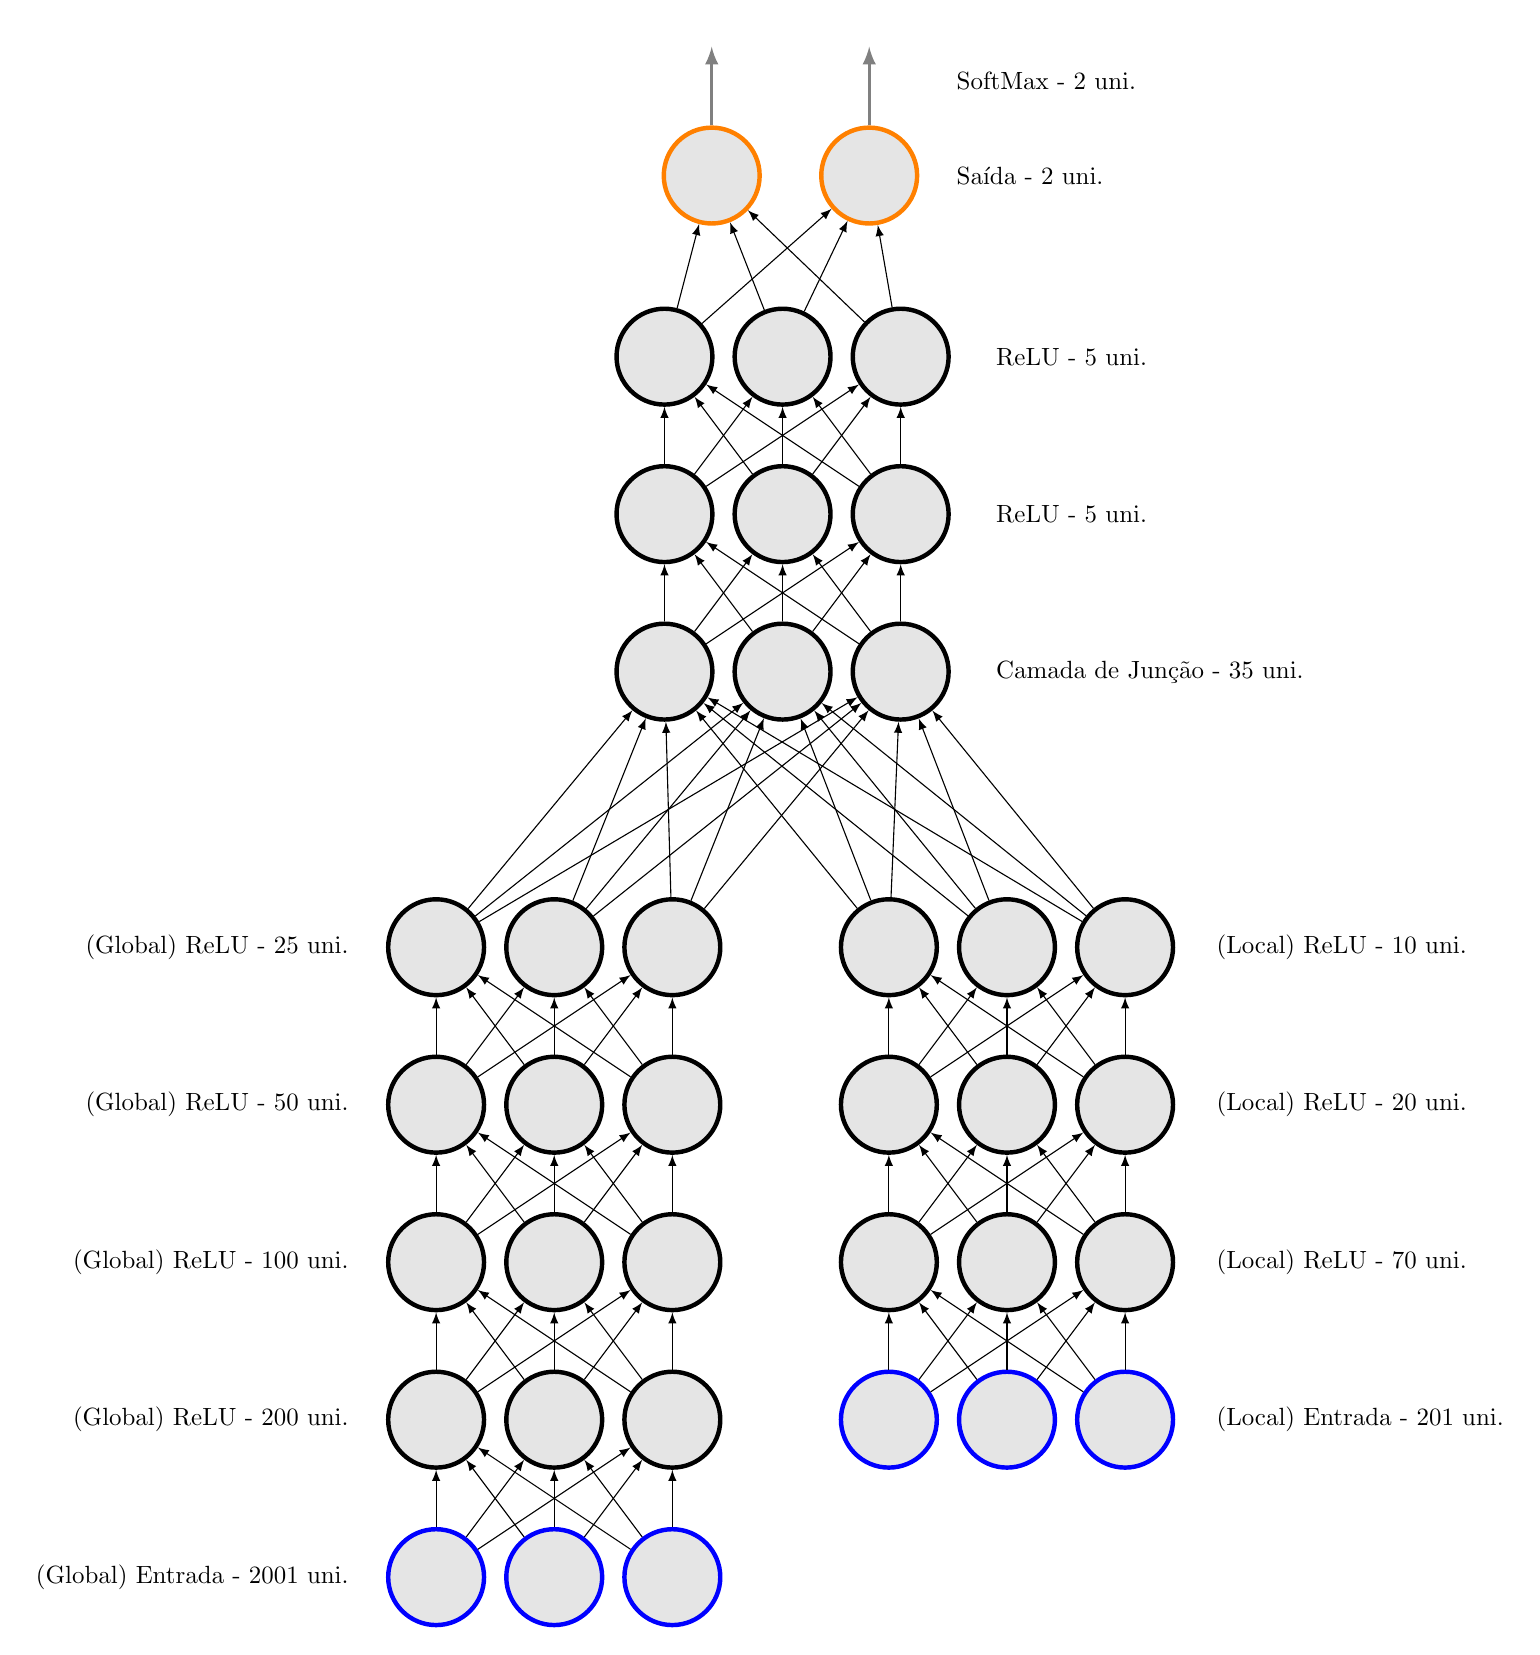
\begin{tikzpicture}
        \tikzstyle{neuronio} = [circle, color=orange, ultra thick, draw, fill=black!10]
    
        \node [neuronio, pin={[pin distance = 10mm, pin edge={-latex, very thick}]above:}] (out-1) at (0,4.3)
        {
        \phantom{$h_{\bm{\theta}}(\bm{x})$}
        };
        
        \node [neuronio, pin={[pin distance = 10mm, pin edge={-latex, very thick}]above:}] (out-2) at (2,4.3)
        {
        \phantom{$h_{\bm{\theta}}(\bm{x})$}
        };
        
        \foreach \i in {1,...,3}
        {   
            [level distance = 3cm, sibling distance = 6cm]
            \node [circle, color=black, ultra thick, draw, fill=black!10] (c3-\i) at (\i*1.5-2.1, 2) {\phantom{$h_{\bm{\theta}}(\bm{x})$}};
            
            \node [circle, color=black, ultra thick, draw, fill=black!10] (c2-\i) at (\i*1.5-2.1, 0) {\phantom{$h_{\bm{\theta}}(\bm{x})$}};
            
            [level distance = 3cm, sibling distance = 6cm]
            \node [circle, color=black, ultra thick, draw, fill=black!10] (c1-\i) at (\i*1.5-2.1, -2) {\phantom{$h_{\bm{\theta}}(\bm{x})$}};
            
            \node [circle, color=black, ultra thick, draw, fill=black!10] (g3-\i) at (\i*1.5-5, -5.5) {\phantom{$h_{\bm{\theta}}(\bm{x})$}};
            
            \node [circle, color=black, ultra thick, draw, fill=black!10] (g2-\i) at (\i*1.5-5, -7.5) {\phantom{$h_{\bm{\theta}}(\bm{x})$}};
             
            \node [circle, color=black, ultra thick, draw, fill=black!10] (g1-\i) at (\i*1.5-5, -9.5) {\phantom{$h_{\bm{\theta}}(\bm{x})$}};
            
            \node [circle, color=black, ultra thick, draw, fill=black!10] (g0-\i) at (\i*1.5-5, -11.5) {\phantom{$h_{\bm{\theta}}(\bm{x})$}};
            
            \node [circle, color=blue, ultra thick, draw, fill=black!10] (g-1-\i) at (\i*1.5-5, -13.5) {\phantom{$h_{\bm{\theta}}(\bm{x})$}};
            
            \node [circle, color=black, ultra thick, draw, fill=black!10] (l3-\i) at (\i*1.5+0.75, -5.5) {\phantom{$h_{\bm{\theta}}(\bm{x})$}};
            
            \node [circle, color=black, ultra thick, draw, fill=black!10] (l2-\i) at (\i*1.5+0.75, -7.5) {\phantom{$h_{\bm{\theta}}(\bm{x})$}};
             
            \node [circle, color=black, ultra thick, draw, fill=black!10] (l1-\i) at (\i*1.5+0.75, -9.5) {\phantom{$h_{\bm{\theta}}(\bm{x})$}};
            
            \node [circle, color=blue, ultra thick, draw, fill=black!10] (l0-\i) at (\i*1.5+0.75, -11.5) {\phantom{$h_{\bm{\theta}}(\bm{x})$}};
        }
        
        
        \foreach \i in {1,...,3}
        {
            \foreach \j in {1,...,3}
            {
                \draw[-latex] (l0-\i) -- (l1-\j);
            }
            \foreach \j in {1,...,3}
            {
                \draw[-latex] (l1-\i) -- (l2-\j);
            }
            \foreach \j in {1,...,3}
            {
                \draw[-latex] (l2-\i) -- (l3-\j);
            }
            \foreach \j in {1,...,3}
            {
                \draw[-latex] (l3-\i) -- (c1-\j);
            }
            
            \foreach \j in {1,...,3}
            {
                \draw[-latex] (g-1-\i) -- (g0-\j);
            }
            \foreach \j in {1,...,3}
            {
                \draw[-latex] (g0-\i) -- (g1-\j);
            }
            \foreach \j in {1,...,3}
            {
                \draw[-latex] (g1-\i) -- (g2-\j);
            }
            \foreach \j in {1,...,3}
            {
                \draw[-latex] (g2-\i) -- (g3-\j);
            }
            \foreach \j in {1,...,3}
            {
                \draw[-latex] (g3-\i) -- (c1-\j);
            }
            
            \foreach \j in {1,...,3}
            {
                \draw[-latex] (c1-\i) -- (c2-\j);
            }
            \foreach \j in {1,...,3}
            {
                \draw[-latex] (c2-\i) -- (c3-\j);
            }
            
            \draw[-latex] (c3-\i) -- (out-1);
            \draw[-latex] (c3-\i) -- (out-2);
        }
        
        \node[right, scale=0.9] at (3, 5.5) {SoftMax - 2 uni.};
        \node[right, scale=0.9] at (3, 4.3) {Saída - 2 uni.};
        \node[right, scale=0.9] at (3.5, 2) {ReLU - 5 uni.};
        \node[right, scale=0.9] at (3.5, 0) {ReLU - 5 uni.};
        \node[right, scale=0.9] at (3.5, -2) {Camada de Junção - 35 uni.};
        
        \node[right, scale=0.9] at (6.3, -5.5) {(Local) ReLU - 10 uni.};
        \node[right, scale=0.9] at (6.3, -7.5) {(Local) ReLU - 20 uni.};
        \node[right, scale=0.9] at (6.3, -9.5) {(Local) ReLU - 70 uni.};
        \node[right, scale=0.9] at (6.3, -11.5) {(Local) Entrada - 201 uni.};
        
        \node[left, scale=0.9] at (-4.5, -5.5) {(Global) ReLU - 25 uni.};
        \node[left, scale=0.9] at (-4.5, -7.5) {(Global) ReLU - 50 uni.};
        \node[left, scale=0.9] at (-4.5, -9.5) {(Global) ReLU - 100 uni.};
        \node[left, scale=0.9] at (-4.5, -11.5) {(Global) ReLU - 200 uni.};
        \node[left, scale=0.9] at (-4.5, -13.5) {(Global) Entrada - 2001 uni.};
        
    \end{tikzpicture}
    }
    \caption*{\small Fonte: Elaboração própria.}
\end{figure}